\documentclass{standalone}
\usepackage{tikz}
\usetikzlibrary{patterns, positioning}

\begin{document}
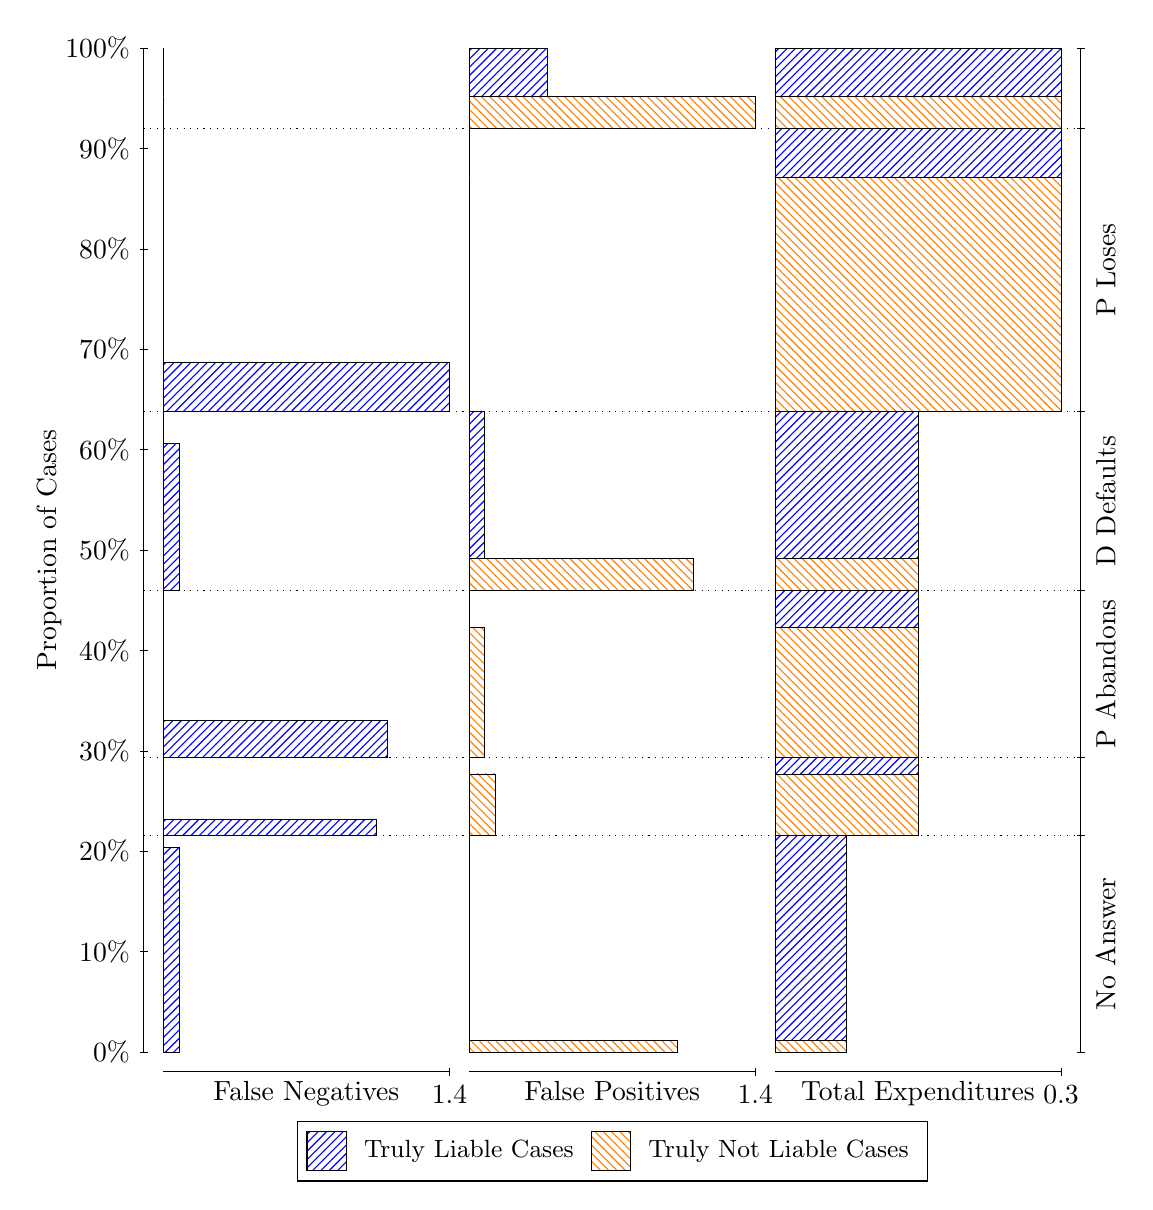
\begin{tikzpicture}
\draw[black, very thin] (1.5,1.75) -- (1.5,14.5);
\node[rotate=90, anchor=center] at (0.3, 8.125) {Proportion of Cases};
\draw[black, very thin] (1.45,1.75) -- (1.55,1.75);
\node[anchor=east] at (1.45, 1.75) {0\%};
\draw[black, very thin] (1.45,3.025) -- (1.55,3.025);
\node[anchor=east] at (1.45, 3.025) {10\%};
\draw[black, very thin] (1.45,4.3) -- (1.55,4.3);
\node[anchor=east] at (1.45, 4.3) {20\%};
\draw[black, very thin] (1.45,5.575) -- (1.55,5.575);
\node[anchor=east] at (1.45, 5.575) {30\%};
\draw[black, very thin] (1.45,6.85) -- (1.55,6.85);
\node[anchor=east] at (1.45, 6.85) {40\%};
\draw[black, very thin] (1.45,8.125) -- (1.55,8.125);
\node[anchor=east] at (1.45, 8.125) {50\%};
\draw[black, very thin] (1.45,9.4) -- (1.55,9.4);
\node[anchor=east] at (1.45, 9.4) {60\%};
\draw[black, very thin] (1.45,10.675) -- (1.55,10.675);
\node[anchor=east] at (1.45, 10.675) {70\%};
\draw[black, very thin] (1.45,11.95) -- (1.55,11.95);
\node[anchor=east] at (1.45, 11.95) {80\%};
\draw[black, very thin] (1.45,13.225) -- (1.55,13.225);
\node[anchor=east] at (1.45, 13.225) {90\%};
\draw[black, very thin] (1.45,14.5) -- (1.55,14.5);
\node[anchor=east] at (1.45, 14.5) {100\%};

\draw[black, very thin] (13.4,1.75) -- (13.4,14.5);
\draw[black, very thin] (13.35,1.75) -- (13.45,1.75);
\node[anchor=west] at (13.35, 1.75) {};
\draw[black, very thin] (13.35,4.4976) -- (13.45,4.4976);
\node[anchor=west] at (13.35, 4.4976) {};
\draw[black, very thin] (13.35,5.4875) -- (13.45,5.4875);
\node[anchor=west] at (13.35, 5.4875) {};
\draw[black, very thin] (13.35,7.6111) -- (13.45,7.6111);
\node[anchor=west] at (13.35, 7.6111) {};
\draw[black, very thin] (13.35,9.8821) -- (13.45,9.8821);
\node[anchor=west] at (13.35, 9.8821) {};
\draw[black, very thin] (13.35,13.481) -- (13.45,13.481);
\node[anchor=west] at (13.35, 13.481) {};
\draw[black, very thin] (13.35,14.5) -- (13.45,14.5);
\node[anchor=west] at (13.35, 14.5) {};

\draw[black, very thin, pattern color=blue, pattern=north east lines] (1.75,1.75) rectangle (1.9482,4.3462);
\draw[black, very thin, pattern color=orange, pattern=north west lines] (1.75,4.3462) rectangle (1.75,4.4976);
\draw[black, very thin, pattern color=blue, pattern=north east lines] (1.75,4.4976) rectangle (4.4585,4.7021);
\draw[black, very thin, pattern color=orange, pattern=north west lines] (1.75,4.7021) rectangle (1.75,5.4875);
\draw[black, very thin, pattern color=blue, pattern=north east lines] (1.75,5.4875) rectangle (4.5906,5.9572);
\draw[black, very thin, pattern color=orange, pattern=north west lines] (1.75,5.9572) rectangle (1.75,7.6111);
\draw[black, very thin, pattern color=blue, pattern=north east lines] (1.75,7.6111) rectangle (1.9482,9.4746);
\draw[black, very thin, pattern color=orange, pattern=north west lines] (1.75,9.4746) rectangle (1.75,9.8821);
\draw[black, very thin, pattern color=blue, pattern=north east lines] (1.75,9.8821) rectangle (5.3833,10.507);
\draw[black, very thin, pattern color=orange, pattern=north west lines] (1.75,10.507) rectangle (1.75,13.481);
\draw[black, very thin, pattern color=orange, pattern=north west lines] (1.75,13.481) rectangle (1.75,13.884);
\draw[black, very thin, pattern color=blue, pattern=north east lines] (1.75,13.884) rectangle (1.75,14.5);
\draw[black, very thin, pattern color=orange, pattern=north west lines] (5.6333,1.75) rectangle (8.2758,1.9014);
\draw[black, very thin, pattern color=blue, pattern=north east lines] (5.6333,1.9014) rectangle (5.6333,4.4976);
\draw[black, very thin, pattern color=orange, pattern=north west lines] (5.6333,4.4976) rectangle (5.9636,5.283);
\draw[black, very thin, pattern color=blue, pattern=north east lines] (5.6333,5.283) rectangle (5.6333,5.4875);
\draw[black, very thin, pattern color=orange, pattern=north west lines] (5.6333,5.4875) rectangle (5.8315,7.1414);
\draw[black, very thin, pattern color=blue, pattern=north east lines] (5.6333,7.1414) rectangle (5.6333,7.6111);
\draw[black, very thin, pattern color=orange, pattern=north west lines] (5.6333,7.6111) rectangle (8.4739,8.0186);
\draw[black, very thin, pattern color=blue, pattern=north east lines] (5.6333,8.0186) rectangle (5.8315,9.8821);
\draw[black, very thin, pattern color=orange, pattern=north west lines] (5.6333,9.8821) rectangle (5.6333,12.856);
\draw[black, very thin, pattern color=blue, pattern=north east lines] (5.6333,12.856) rectangle (5.6333,13.481);
\draw[black, very thin, pattern color=orange, pattern=north west lines] (5.6333,13.481) rectangle (9.2667,13.884);
\draw[black, very thin, pattern color=blue, pattern=north east lines] (5.6333,13.884) rectangle (6.6242,14.5);
\draw[black, very thin, pattern color=orange, pattern=north west lines] (9.5167,1.75) rectangle (10.425,1.9014);
\draw[black, very thin, pattern color=blue, pattern=north east lines] (9.5167,1.9014) rectangle (10.425,4.4976);
\draw[black, very thin, pattern color=orange, pattern=north west lines] (9.5167,4.4976) rectangle (11.333,5.283);
\draw[black, very thin, pattern color=blue, pattern=north east lines] (9.5167,5.283) rectangle (11.333,5.4875);
\draw[black, very thin, pattern color=orange, pattern=north west lines] (9.5167,5.4875) rectangle (11.333,7.1414);
\draw[black, very thin, pattern color=blue, pattern=north east lines] (9.5167,7.1414) rectangle (11.333,7.6111);
\draw[black, very thin, pattern color=orange, pattern=north west lines] (9.5167,7.6111) rectangle (11.333,8.0186);
\draw[black, very thin, pattern color=blue, pattern=north east lines] (9.5167,8.0186) rectangle (11.333,9.8821);
\draw[black, very thin, pattern color=orange, pattern=north west lines] (9.5167,9.8821) rectangle (13.15,12.856);
\draw[black, very thin, pattern color=blue, pattern=north east lines] (9.5167,12.856) rectangle (13.15,13.481);
\draw[black, very thin, pattern color=orange, pattern=north west lines] (9.5167,13.481) rectangle (13.15,13.884);
\draw[black, very thin, pattern color=blue, pattern=north east lines] (9.5167,13.884) rectangle (13.15,14.5);
\draw[black, dotted] (1.5,4.4976) -- (13.4,4.4976);
\draw[black, dotted] (1.5,5.4875) -- (13.4,5.4875);
\draw[black, dotted] (1.5,7.6111) -- (13.4,7.6111);
\draw[black, dotted] (1.5,9.8821) -- (13.4,9.8821);
\draw[black, dotted] (1.5,13.481) -- (13.4,13.481);
\draw[black, very thin] (1.75,1.5) -- (5.3833,1.5);
\node[anchor=north] at (3.5667, 1.5) {False Negatives};
\draw[black, very thin] (5.3833,1.45) -- (5.3833,1.55);
\node[anchor=north] at (5.3833, 1.45) {1.4};

\draw[black, very thin] (5.6333,1.5) -- (9.2667,1.5);
\node[anchor=north] at (7.45, 1.5) {False Positives};
\draw[black, very thin] (9.2667,1.45) -- (9.2667,1.55);
\node[anchor=north] at (9.2667, 1.45) {1.4};

\draw[black, very thin] (9.5167,1.5) -- (13.15,1.5);
\node[anchor=north] at (11.333, 1.5) {Total Expenditures};
\draw[black, very thin] (13.15,1.45) -- (13.15,1.55);
\node[anchor=north] at (13.15, 1.45) {0.3};

\node[black, centered, rotate=90] at (13.72, 3.1238) {No Answer};

\node[black, centered, rotate=90] at (13.72, 6.5493) {P Abandons};
\node[black, centered, rotate=90] at (13.72, 8.7466) {D Defaults};
\node[black, centered, rotate=90] at (13.72, 11.682) {P Loses};


\draw (7.449999999999999,1.5) node[draw=none] (baseCoordinate) {};
\begin{scope}[align=center]
        \matrix[scale=0.5, draw=black, below=0.5cm of baseCoordinate, nodes={draw}, column sep=0.1cm]{
            \node[rectangle, draw, minimum width=0.5cm, minimum height=0.5cm, pattern=north east lines, pattern color=blue] {}; &
            \node[draw=none, font=\small] (B) {Truly Liable Cases}; &
            \node[rectangle, draw, minimum width=0.5cm, minimum height=0.5cm, pattern=north west lines, pattern color=orange] {}; &
            \node[draw=none, font=\small] (B) {Truly Not Liable Cases}; \\
            };
\end{scope}

\end{tikzpicture}
\end{document}